\documentclass[11pt,a4paper]{article}
\usepackage[T1]{fontenc}\usepackage{lmodern}
\usepackage[margin=22mm,headheight=14pt]{geometry}
\usepackage{amsmath,amssymb,bm,booktabs,tabularx,array,graphicx,float,fancyhdr,microtype,xcolor}
\usepackage[colorlinks=true,linkcolor=blue!45!black,urlcolor=blue!45!black,citecolor=blue!45!black]{hyperref}
\setlength{\parindent}{0pt}\setlength{\parskip}{5pt}\renewcommand{\arraystretch}{1.15}
\pagestyle{fancy}\fancyhf{}\fancyhead[L]{\small QFT Project B | Step 4}\fancyhead[R]{\small Group B}\fancyfoot[C]{\thepage}
\newcommand{\dd}{\mathrm{d}}
\begin{document}\hypersetup{pageanchor=false}
\begin{titlepage}\centering\vspace*{3mm}

\includegraphics[width=36mm]{assets/bits_logo.png}\par\vspace{13mm}
{\Large\bfseries BITS PILANI K.K. BIRLA GOA CAMPUS\par}\vspace{3mm}
{\large\bfseries Department of Physics\par}\vspace{18mm}
{\LARGE\bfseries What Quantum Trace Can\\[2mm] a Heavy Particle Leave?\par}\vspace{6mm}
{\large Curvature--Spectator Entanglement\\and the Cosmological Collider\par}\vspace{10mm}
{\large\bfseries Step 4: Initial States and Free Modes\par}\vspace{17mm}
{\Large\bfseries Group-B\par}\vspace{5mm}
\begin{tabular}{ll}Priyansh Rawat & 2023B5A70968G\\Mayank Sinha & 2023B5A70942G\\Samarth Bhatnagar & 2023B5A70853G\end{tabular}
\vfill{\large Under Professor: Rudranil Basu\par}\vspace{7mm}{29 October 2026\par}
\end{titlepage}\setcounter{page}{1}\hypersetup{pageanchor=true}
\section{Free modes and canonical initial data}
At zero mixing the Bunch--Davies light mode and momentum are
\begin{equation}Q_{\rm BD}=\frac{(1-ix)e^{ix}}{\sqrt2},\qquad\Pi_{q,\rm BD}=-\frac{e^{ix}}{\sqrt2 x}.\end{equation}
For the spectator,
\begin{equation}\Sigma_{\rm BD}=\frac{\sqrt\pi}{2}e^{i\pi(\nu/2+1/4)}x^{3/2}H_\nu^{(1)}(x),\quad\nu=\sqrt{9/4-M^2},\quad\Pi_{\sigma,\rm BD}=-\Sigma'_{\rm BD}/x^2.\end{equation}
For $M>3/2$, $\nu$ is imaginary. We evaluate the Hankel functions with complex-order support and use $H_\nu'=(H_{\nu-1}-H_{\nu+1})/2$. The exponential prefactor supplies the required normalisation.
At a finite initial $X$, the product initial state has canonical columns $(Q,\Pi_q,0,0)^T$ and $(0,0,\Sigma,\Pi_\sigma)^T$. In the velocity form, $\dot Q=x^3\Pi_q-g\Sigma$, so the second column starts with $\dot Q=-g\Sigma$.
The free analytic/numerical comparison on $10^{-3}\le x\le100$ gives maximum scaled complex errors $5.805\times10^{-10}$ (light) and $5.860\times10^{-10}$ (heavy). The late light power is $0.5000005$, consistent with $(1+x^2)/2\to1/2$.
\begin{figure}[H]\centering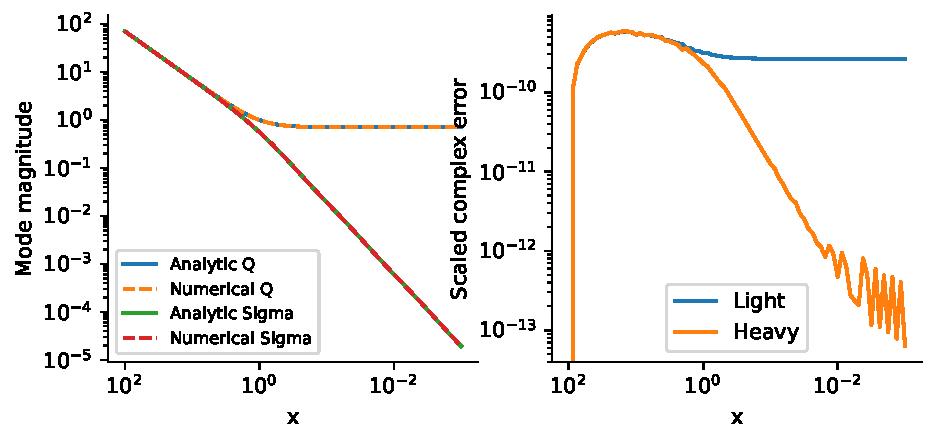
\includegraphics[width=.91\linewidth]{figures/free_modes.pdf}\caption{Free analytic and numerical mode magnitudes, together with errors in the complex modes.}\end{figure}
\newpage
\section{Starting-time and commutator checks}
With rows $(Q,\Pi_q,\Sigma,\Pi_\sigma)$, form $W=\mathcal M\mathcal M^\dagger$ and test $2\operatorname{Im}W=\Omega$, where $\Omega=\operatorname{diag}(J,J)$ and $J_{12}=1$, $J_{21}=-1$. We require a maximum entrywise residual below $10^{-6}$ on the interval used for entropy. The free test reaches $5.225\times10^{-7}$. No final covariance renormalisation is applied.
\begin{figure}[H]\centering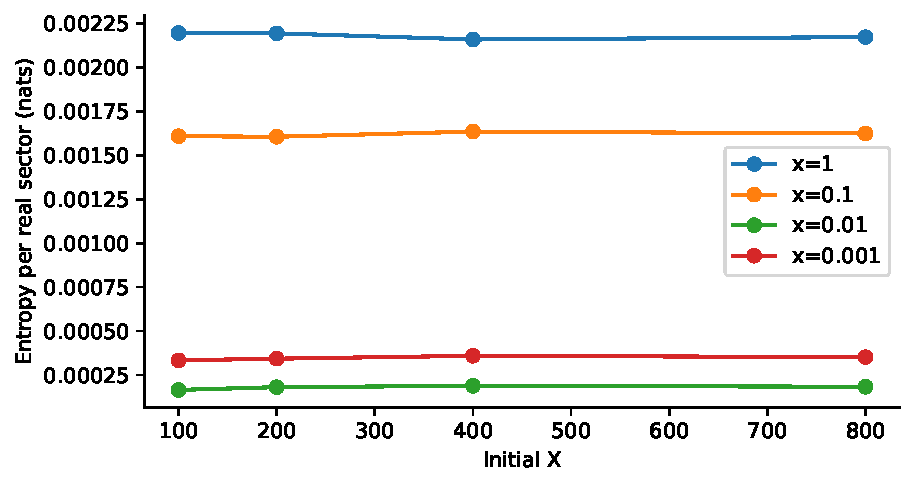
\includegraphics[width=.91\linewidth]{figures/initial_time_convergence.pdf}\caption{Finite-time product-state entropy under increasing initial $X$. These are diagnostic runs; late samples that fail the commutator criterion are not used as production entropy results.}\end{figure}The product-state limit is slow enough to matter for the much smaller bispectrum. We therefore also test a positive-frequency ultraviolet initial state, obtained from an asymptotic Riccati expansion. Its position covariance and momentum relation enforce the canonical initial commutators; it is not a correction imposed on the evolved state. Step 8 derives this construction.
The saved adiabatic table compares orders 4 and 6 at $X=100,200,400,800$, including both power and entropy. At $x=0.01$, the sixth-order entropy is approximately $1.845987\times10^{-4}$ across these starting times. The production Gaussian scan uses order 6, $X=400$ and tighter tolerances $2.5\times10^{-14}/10^{-17}$.\begin{thebibliography}{9}\small
\bibitem{chen} X. Chen and Y. Wang, \emph{Quasi-Single Field Inflation and Non-Gaussianities}, JCAP 04 (2010) 027, \href{https://arxiv.org/abs/0911.3380}{arXiv:0911.3380}.\end{thebibliography}
\textbf{Code and supporting data:} \href{https://github.com/rawatpriyansh17/QFT-PROJECT-GROUP-B/tree/main/step4}{step4 on GitHub}.\newpage\section*{Contributions (equal)}\begin{center}\begin{tabularx}{\linewidth}{p{33mm}X}\toprule Member & Contribution\\\midrule Priyansh Rawat & Bunch--Davies modes and initial-state conventions.\\[3mm]Samarth Bhatnagar & Canonical commutator and starting-time checks.\\[3mm]Mayank Sinha & Free-mode implementation, adiabatic tests and figures.\\\bottomrule\end{tabularx}\end{center}\end{document}